% !TEX root = ../main.tex
\chapter{质量与配置保障计划}

\section{质量保证措施}

\subsection{质量管理框架}

本项目采用\textbf{全生命周期质量管理}理念\cite{pressman2014software}，在各阶段嵌入质量控制点，如图~\ref{fig:quality_framework}所示。

\begin{figure}[htbp]
    \centering
    \begin{tikzpicture}[
            node distance=1.5cm,
            phase/.style={rectangle, draw, rounded corners, minimum width=2cm, minimum height=1cm, align=center, font=\small},
            quality/.style={rectangle, draw, dashed, minimum width=2cm, minimum height=0.6cm, align=center, font=\footnotesize, fill=yellow!20},
            arrow/.style={->, >=stealth, thick}
        ]
        % 阶段
        \node[phase, fill=blue!20] (req) {需求分析};
        \node[phase, fill=green!20, right=of req] (design) {系统设计};
        \node[phase, fill=orange!20, right=of design] (dev) {编码实现};
        \node[phase, fill=purple!20, right=of dev] (test) {测试验证};
        \node[phase, fill=red!20, right=of test] (deploy) {部署运维};

        % 质量控制点
        \node[quality, below=0.8cm of req] (q1) {需求评审};
        \node[quality, below=0.8cm of design] (q2) {设计评审};
        \node[quality, below=0.8cm of dev] (q3) {代码评审};
        \node[quality, below=0.8cm of test] (q4) {测试验收};
        \node[quality, below=0.8cm of deploy] (q5) {运维监控};

        % 箭头
        \draw[arrow] (req) -- (design);
        \draw[arrow] (design) -- (dev);
        \draw[arrow] (dev) -- (test);
        \draw[arrow] (test) -- (deploy);

        \draw[arrow, dashed] (req) -- (q1);
        \draw[arrow, dashed] (design) -- (q2);
        \draw[arrow, dashed] (dev) -- (q3);
        \draw[arrow, dashed] (test) -- (q4);
        \draw[arrow, dashed] (deploy) -- (q5);
    \end{tikzpicture}
    \caption{全生命周期质量管理框架}
    \label{fig:quality_framework}
\end{figure}

\subsection{代码质量标准}

表~\ref{tab:code_standards}定义了项目的代码质量标准。

\begin{table}[htbp]
    \centering
    \caption{代码质量标准}
    \label{tab:code_standards}
    \begin{tabular}{p{3cm}p{4cm}p{5cm}}
        \toprule
        \textbf{维度} & \textbf{标准}                 & \textbf{检查工具}                  \\
        \midrule
        代码风格        & PEP 8 (Python) / Dart Style & flake8, dart analyze           \\
        类型检查        & 类型注解覆盖率 $\geq 80\%$         & mypy, dart --enable-experiment \\
        注释规范        & 公共API必须有docstring           & pydocstyle                     \\
        复杂度控制       & 圈复杂度 $\leq 15$              & radon                          \\
        重复代码        & 重复率 $\leq 5\%$              & 人工审查                           \\
        \bottomrule
    \end{tabular}
\end{table}

\section{测试策略}

\subsection{测试金字塔}

项目遵循测试金字塔原则\cite{sommerville2015software}，如图~\ref{fig:test_pyramid}所示。

\begin{figure}[H]
    \centering
    \begin{tikzpicture}[
            level/.style={trapezium, draw, trapezium angle=70, minimum width=2cm, align=center, font=\small}
        ]
        % 金字塔层
        \node[level, fill=green!30, minimum width=8cm] (unit) at (0, 0) {单元测试 (Unit Tests)};
        \node[level, fill=yellow!30, minimum width=5cm] (int) at (0, 1.5) {集成测试 (Integration)};
        \node[level, fill=orange!30, minimum width=3cm] (e2e) at (0, 2.8) {E2E测试};

        % 标注
        \node[right, font=\footnotesize] at (4.5, 0) {数量最多、速度最快};
        \node[right, font=\footnotesize] at (3, 1.5) {API接口验证};
        \node[right, font=\footnotesize] at (2, 2.8) {用户场景验证};
    \end{tikzpicture}
    \caption{测试金字塔策略}
    \label{fig:test_pyramid}
\end{figure}

\subsection{单元测试}

单元测试覆盖后端核心模块，使用pytest框架：

\begin{lstlisting}[language=Python, caption=单元测试示例]
class TestEnergyOptimizer:
    def test_optimize_basic_scenario(self):
        """测试基础优化场景"""
        optimizer = EnergyOptimizer(
            battery_capacity=10.0,
            max_power=3.0
        )
        load = [5.0] * 24
        prices = [0.3]*8 + [0.6]*10 + [1.0]*4 + [0.3]*2
        
        result = optimizer.optimize(load, prices, initial_soc=0.5)
        
        assert result['status'] == 'optimal'
        assert result['total_cost'] < sum(load) * 0.6
        assert all(0 <= soc <= 1 for soc in result['soc'])
\end{lstlisting}

\subsection{集成测试}

集成测试验证API接口的端到端行为：

\begin{table}[H]
    \centering
    \caption{关键API接口测试用例}
    \label{tab:api_tests}
    \begin{tabularx}{\textwidth}{l l l X}
        \toprule
        \textbf{测试ID} & \textbf{接口}                & \textbf{测试场景} & \textbf{预期结果}    \\
        \midrule
        IT-01         & POST /api/auth/verify      & 有效Token       & 返回200, user信息    \\
        IT-02         & POST /api/auth/verify      & 无效Token       & 返回401错误          \\
        IT-03         & POST /api/optimization/run & 正常参数          & 返回优化结果           \\
        IT-04         & POST /api/optimization/run & SOC超出范围       & 返回400校验错误        \\
        IT-05         & GET /api/health            & 健康检查          & 返回200, status=ok \\
        \bottomrule
    \end{tabularx}
\end{table}

\section{验收标准}

\subsection{功能验收}

表~\ref{tab:acceptance_func}定义了功能验收标准。

\begin{table}[htbp]
    \centering
    \caption{功能验收标准}
    \label{tab:acceptance_func}
    \begin{tabular}{lp{5cm}p{4cm}c}
        \toprule
        \textbf{编号} & \textbf{验收项} & \textbf{验收标准}    & \textbf{权重} \\
        \midrule
        AC-01       & 用户登录功能       & 支持邮箱和Google登录    & 10\%        \\
        AC-02       & 负载预测功能       & 预测结果在3秒内返回       & 20\%        \\
        AC-03       & 储能优化功能       & 返回OPTIMAL状态的调度计划 & 30\%        \\
        AC-04       & 结果可视化        & 图表正确渲染，动画流畅      & 15\%        \\
        AC-05       & 数据分析功能       & 支持CSV/Excel上传分析  & 15\%        \\
        AC-06       & 系统稳定性        & 连续运行24h无崩溃       & 10\%        \\
        \bottomrule
    \end{tabular}
\end{table}

\subsection{性能验收}

\begin{table}[htbp]
    \centering
    \caption{性能验收标准}
    \label{tab:acceptance_perf}
    \begin{tabular}{lp{5cm}c}
        \toprule
        \textbf{指标} & \textbf{验收标准}             & \textbf{测试方法}    \\
        \midrule
        API响应时间     & P95 $\leq 500$ ms (非优化接口) & 压力测试             \\
        优化求解时间      & 单次 $\leq 5$ s             & 功能测试             \\
        页面加载时间      & 首屏 $\leq 3$ s (3G网络)      & Lighthouse       \\
        内存占用        & 后端实例 $\leq 512$ MB        & Cloud Monitoring \\
        \bottomrule
    \end{tabular}
\end{table}

\section{配置管理}

\subsection{版本控制策略}

项目采用\textbf{Git Flow}分支策略，如图~\ref{fig:git_flow}所示。

\begin{figure}[H]
    \centering
    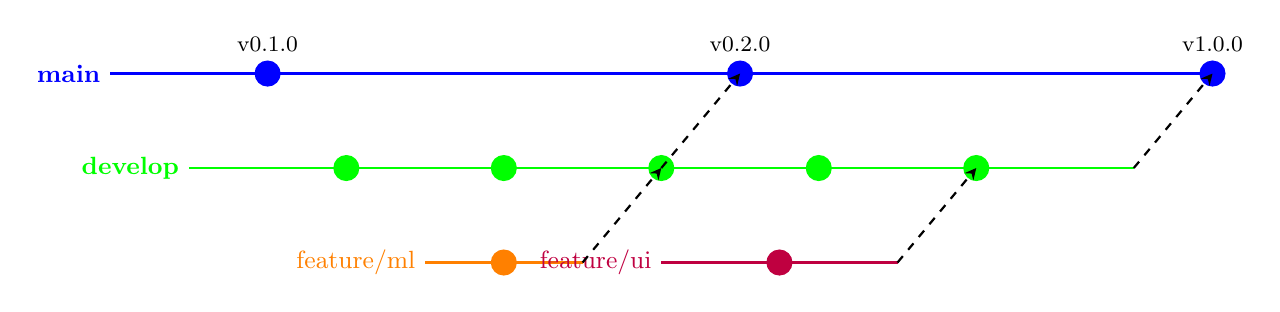
\begin{tikzpicture}[
            x=1cm, y=0.8cm,
            branch/.style={thick},
            commit/.style={circle, fill, minimum size=0.3cm},
            merge/.style={->, >=stealth, thick}
        ]
        % main分支
        \draw[branch, blue] (0, 0) -- (14, 0);
        \node[left, font=\small\bfseries, blue] at (0, 0) {main};
        \foreach \x in {2, 8, 14} {
                \node[commit, blue] at (\x, 0) {};
            }

        % develop分支
        \draw[branch, green] (1, -1.5) -- (13, -1.5);
        \node[left, font=\small\bfseries, green] at (1, -1.5) {develop};
        \foreach \x in {3, 5, 7, 9, 11} {
                \node[commit, green] at (\x, -1.5) {};
            }

        % feature分支
        \draw[branch, orange] (4, -3) -- (6, -3);
        \node[left, font=\small, orange] at (4, -3) {feature/ml};
        \node[commit, orange] at (5, -3) {};

        \draw[branch, purple] (7, -3) -- (10, -3);
        \node[left, font=\small, purple] at (7, -3) {feature/ui};
        \node[commit, purple] at (8.5, -3) {};

        % 合并箭头
        \draw[merge, dashed] (6, -3) -- (7, -1.5);
        \draw[merge, dashed] (10, -3) -- (11, -1.5);
        \draw[merge, dashed] (7, -1.5) -- (8, 0);
        \draw[merge, dashed] (13, -1.5) -- (14, 0);

        % 版本标签
        \node[above, font=\footnotesize] at (2, 0.2) {v0.1.0};
        \node[above, font=\footnotesize] at (8, 0.2) {v0.2.0};
        \node[above, font=\footnotesize] at (14, 0.2) {v1.0.0};
    \end{tikzpicture}
    \caption{Git Flow 分支策略}
    \label{fig:git_flow}
\end{figure}

\subsection{分支命名规范}

\begin{table}[htbp]
    \centering
    \caption{分支命名规范}
    \label{tab:branch_naming}
    \begin{tabular}{lp{4cm}l}
        \toprule
        \textbf{分支类型} & \textbf{命名格式} & \textbf{示例}         \\
        \midrule
        主分支           & main          & main                \\
        开发分支          & develop       & develop             \\
        功能分支          & feature/<功能名> & feature/ml-training \\
        修复分支          & fix/<问题描述>    & fix/api-timeout     \\
        发布分支          & release/<版本号> & release/v1.0.0      \\
        \bottomrule
    \end{tabular}
\end{table}

\subsection{提交信息规范}

采用Conventional Commits规范：

\begin{lstlisting}[caption=Git提交信息格式]
<type>(<scope>): <subject>

[optional body]

[optional footer]
\end{lstlisting}

类型（type）包括：
\begin{itemize}
    \item \texttt{feat}: 新功能
    \item \texttt{fix}: Bug修复
    \item \texttt{docs}: 文档更新
    \item \texttt{refactor}: 代码重构
    \item \texttt{test}: 测试相关
    \item \texttt{chore}: 构建/工具链
\end{itemize}

\section{文档管理}

\subsection{文档分类}

表~\ref{tab:doc_types}列出了项目文档分类及管理要求。

\begin{table}[htbp]
    \centering
    \caption{项目文档分类与管理}
    \label{tab:doc_types}
    \begin{tabular}{llll}
        \toprule
        \textbf{文档类型} & \textbf{格式} & \textbf{存储位置} & \textbf{更新频率} \\
        \midrule
        需求文档          & LaTeX/PDF   & GitHub仓库      & 按里程碑          \\
        设计文档          & LaTeX/PDF   & GitHub仓库      & 按里程碑          \\
        API文档         & Markdown    & 代码仓库/docs     & 随代码更新         \\
        用户手册          & PDF         & 发布包           & 按版本           \\
        会议记录          & Markdown    & 共享文档          & 每次会议后         \\
        \bottomrule
    \end{tabular}
\end{table}

\subsection{备份策略}

\begin{enumerate}
    \item \textbf{代码备份}：GitHub远程仓库 + 本地克隆
    \item \textbf{数据备份}：Firebase自动备份（每日）
    \item \textbf{文档备份}：Google Drive同步
\end{enumerate}